\documentclass[12pt,a4paper]{article}

% Language and encoding
\usepackage[utf8]{inputenc}
\usepackage[T1]{fontenc}
\usepackage[english]{babel}

% Geometry
\usepackage[margin=1in,top=1.2in,bottom=1.2in]{geometry}

% Mathematics
\usepackage{amsmath,amssymb}

% Graphics and color
\usepackage{graphicx}
\usepackage{xcolor}
\usepackage{float}

% Tables
\usepackage{booktabs}
\usepackage{makecell}
\usepackage{array}

% Hyperlinks
\usepackage{hyperref}
\hypersetup{
    colorlinks=true,
    linkcolor=blue,
    citecolor=blue,
    urlcolor=blue
}

% Captions and subfigures
\usepackage{caption}
\usepackage{subcaption}

% Header/footer
\usepackage{fancyhdr}
\pagestyle{fancy}
\fancyhf{}
\fancyhead[L]{\small Machine Learning-Based Clinical Decision Support for Diabetes Prediction}
\fancyhead[R]{\small B.Sc. Thesis}
\fancyfoot[C]{\thepage}

% Title page information
\title{\textbf{Machine Learning-Based Clinical Decision Support for Diabetes Prediction}\\ \large A Re-Implementation and Comprehensive Analysis}
\author{\textbf{Pouyan Fallahi}\\[2mm] \small B.Sc. in Computer Engineering \\ \small Azad University, South Tehran Campus, Tehran, Iran \\ \small \texttt{fallahipouyan78@gmail.com} \\[3mm] \small Supervisor: Dr. Razieh Farazkish}
\date{Academic Year 2021--2022}

\begin{document}

\maketitle
\thispagestyle{empty}

\begin{abstract}
Diabetes mellitus is a chronic metabolic disorder with severe long-term complications. Early detection can significantly improve patient outcomes, but manual screening is resource-intensive. In this thesis, we re-implement and critically evaluate a machine learning-based clinical decision support system for diabetes prediction using the Pima Indians Diabetes Dataset. Following a rigorous pipeline of data preprocessing (zero-imputation, scaling), dual-method feature selection (SelectKBest and Recursive Feature Elimination), and three supervised classifiers---Logistic Regression, Decision Tree, and Support Vector Machine (SVM)---we achieve a maximum accuracy of 71.4\% and recall of 53.7\%. The study highlights the crucial trade-off between precision and recall in medical screening, discusses the clinical relevance of selected features (Glucose, BMI, Pregnancies, Age), and provides a reproducible framework for future enhancements. The work demonstrates a thorough understanding of end-to-end machine learning pipelines, from raw data to actionable clinical insights.
\end{abstract}

\newpage
\tableofcontents
\newpage

\section{Introduction}
\label{sec:introduction}

Diabetes is a global health epidemic, affecting over 400 million people worldwide. Early diagnosis and intervention are key to preventing complications such as neuropathy, retinopathy, and cardiovascular disease. Clinical decision support systems (CDSS) powered by machine learning can assist healthcare professionals by identifying high-risk individuals from routine medical data.

This project re-implements the core machine learning pipeline of a B.Sc. thesis that originally employed Logistic Regression, Decision Trees, and SVM for diabetes prediction. The objectives are:
\begin{itemize}
    \item To demonstrate a complete, reproducible ML workflow.
    \item To critically evaluate model performance using clinically relevant metrics (accuracy, precision, recall).
    \item To identify the most important risk factors through dual-method feature selection.
\end{itemize}

The report is structured as follows: Section~\ref{sec:dataset} describes the dataset; Section~\ref{sec:methodology} details the methodology; Section~\ref{sec:results} presents the experimental results; Section~\ref{sec:discussion} provides a clinical interpretation and discussion; Section~\ref{sec:conclusion} concludes with future work.

\section{Dataset Description}
\label{sec:dataset}

The \textbf{Pima Indians Diabetes Database} (originally from the National Institute of Diabetes and Digestive and Kidney Diseases) is a benchmark binary classification task. It contains \textbf{768} female patients (at least 21 years old of Pima Indian heritage) with \textbf{8} medical predictors and a binary outcome indicating whether the patient developed diabetes within five years.

\begin{table}[H]
\centering
\caption{Feature descriptions}
\label{tab:features}
\begin{tabular}{ll}
\toprule
\textbf{Feature} & \textbf{Description} \\
\midrule
Pregnancies & Number of times pregnant \\
Glucose & Plasma glucose concentration (2-hour OGTT) \\
BloodPressure & Diastolic blood pressure (mm Hg) \\
SkinThickness & Triceps skin fold thickness (mm) \\
Insulin & 2-Hour serum insulin (mu U/ml) \\
BMI & Body mass index (kg/m$^2$) \\
DiabetesPedigreeFunction & Diabetes pedigree function (genetic risk score) \\
Age & Age (years) \\
\textbf{Outcome} & \textbf{1 -- Diabetes, 0 -- No diabetes} \\
\bottomrule
\end{tabular}
\end{table}

The dataset exhibits a moderate class imbalance: 34.9\% positive cases, making accuracy alone an insufficient metric.

\section{Methodology}
\label{sec:methodology}

The overall workflow follows the standard machine learning pipeline:
\begin{enumerate}
    \item \textbf{Data Preprocessing} -- Handle missing values encoded as zeros and scale features.
    \item \textbf{Feature Selection} -- Combine univariate filtering (SelectKBest) with model-based recursive elimination (RFE) to obtain a concise, clinically meaningful feature set.
    \item \textbf{Model Training} -- Train three classifiers (Logistic Regression, Decision Tree, SVM) on the selected features.
    \item \textbf{Evaluation} -- Assess performance using accuracy, precision, recall, and confusion matrices, with recall prioritised for a screening tool.
\end{enumerate}

All random states are fixed (\texttt{random\_state=42}) for reproducibility.

\subsection{Data Preprocessing}

Several features contain \textbf{physiologically impossible zeros} (e.g., Glucose, BloodPressure, BMI) which are treated as missing. We replace zeros with \texttt{NaN} and impute using the \textbf{median}, which is robust to outliers. The columns \texttt{Pregnancies}, \texttt{DiabetesPedigreeFunction}, and \texttt{Age} have valid zero values consistent with medical records.

After imputation, all features are standardised to zero mean and unit variance via \texttt{StandardScaler}. This step is essential for distance-based models (SVM, Logistic Regression) and does not affect tree-based models.

Original distributions and imputed statistics are shown in Figure~\ref{fig:histograms}.

\begin{figure}[H]
    \centering
    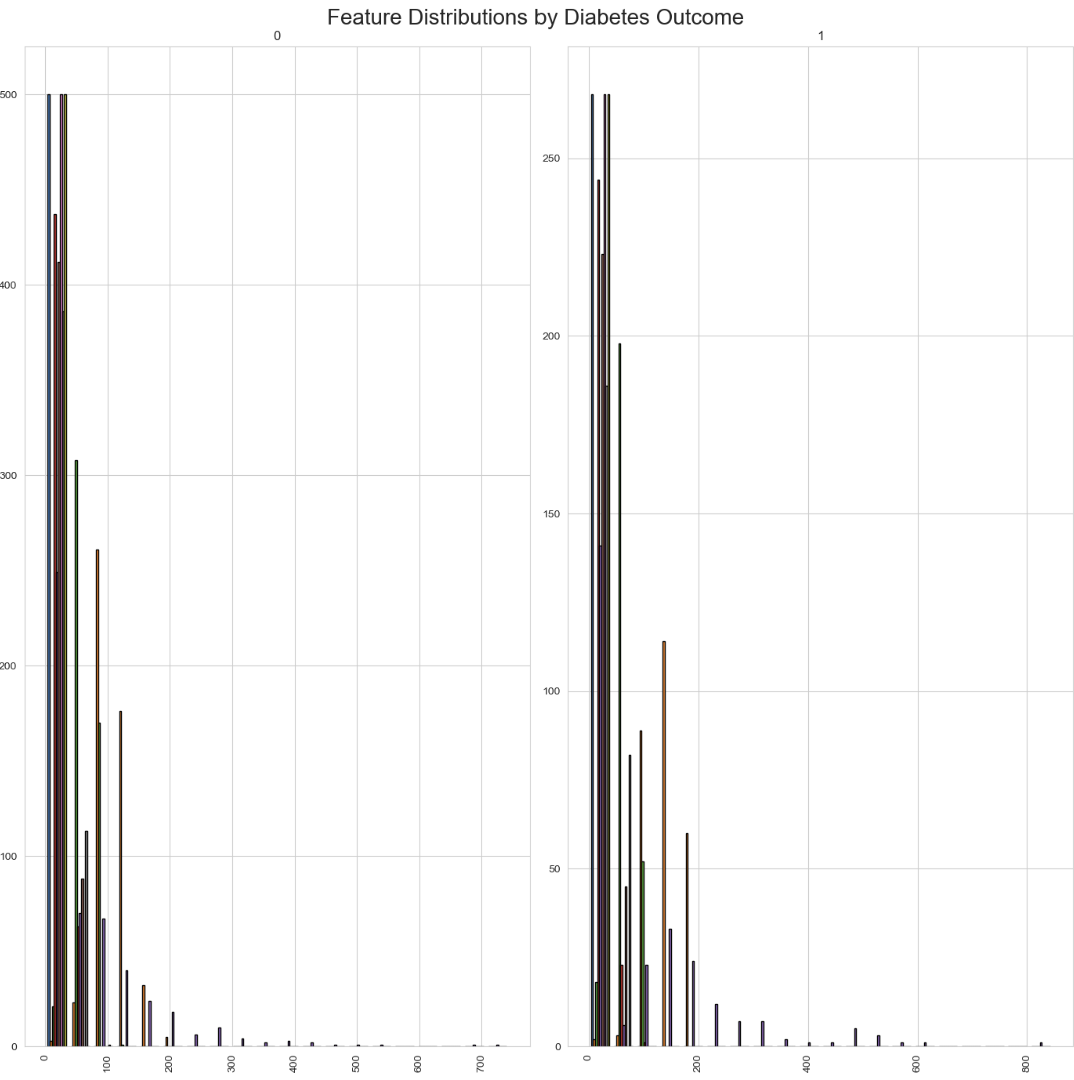
\includegraphics[width=0.95\textwidth]{histograms.png}
    \caption{Feature distributions by diabetes outcome. The presence of invalid zeros in Glucose, BloodPressure, SkinThickness, Insulin, and BMI is evident.}
    \label{fig:histograms}
\end{figure}

\subsection{Feature Selection}

To improve model interpretability and reduce overfitting, we employ two complementary feature selection techniques:
\begin{itemize}
    \item \textbf{SelectKBest} with the ANOVA F-value: ranks features by their univariate correlation with the target.
    \item \textbf{Recursive Feature Elimination (RFE)} with Logistic Regression: iteratively removes the least important feature based on model coefficients.
\end{itemize}

We set $k=6$ (top six features) for each method and then take the \textbf{intersection} of the two selected sets. This conservative approach ensures that only features consistently identified by both statistical and model-based criteria are retained.

The agreement between methods yields a concise set of \textbf{four risk factors}: \emph{Pregnancies}, \emph{Glucose}, \emph{BMI}, and \emph{Age}. All are well-accepted clinical predictors of diabetes, making the model not only effective but also interpretable in a healthcare setting.

\subsection{Model Training and Evaluation}
\label{subsec:evaluation}

The data is split into 80\% training and 20\% test sets, stratified to preserve the class distribution. Three classifiers are trained:
\begin{itemize}
    \item \textbf{Logistic Regression} -- linear baseline, directly interpretable probabilities.
    \item \textbf{Decision Tree} -- non-linear, captures complex interactions.
    \item \textbf{SVM} with RBF kernel -- effective with high-dimensional decision boundaries, even on few features.
\end{itemize}

Evaluation metrics are accuracy, precision, recall, and the confusion matrix. In a screening context, \textbf{recall} (sensitivity) is the most critical measure, as missing a diabetic patient can have severe health consequences.

\section{Results and Analysis}
\label{sec:results}

\subsection{Performance Summary}

Table~\ref{tab:perf} and Figure~\ref{fig:bar} present the performance of each model. Logistic Regression achieves the highest recall (53.7\%), while SVM exhibits the highest precision (61.4\%).

\begin{table}[H]
\centering
\caption{Model performance on the test set}
\label{tab:perf}
\begin{tabular}{lccc}
\toprule
\textbf{Model} & \textbf{Accuracy} & \textbf{Precision} & \textbf{Recall} \\
\midrule
Logistic Regression & 0.708 & 0.592 & \textbf{0.537} \\
Decision Tree       & 0.682 & 0.547 & \textbf{0.537} \\
SVM                 & 0.714 & \textbf{0.614} & 0.500 \\
\bottomrule
\end{tabular}
\par\smallskip
\small \emph{High recall is preferred in diabetes screening; high precision reduces false alarms.}
\end{table}

\begin{figure}[H]
    \centering
    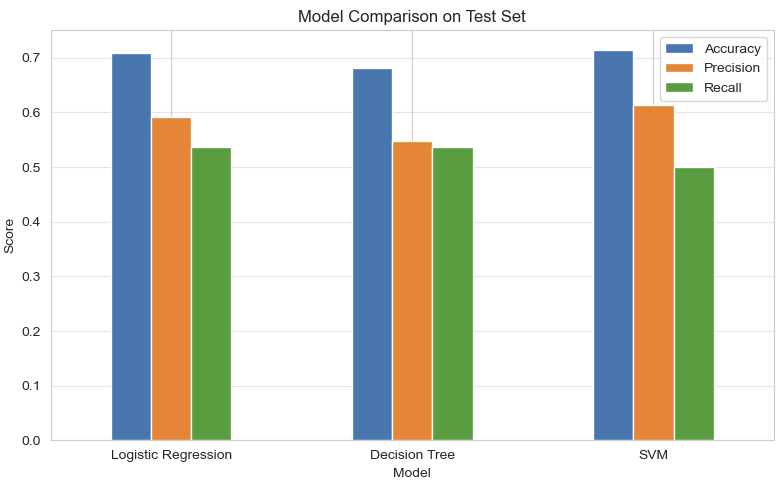
\includegraphics[width=0.9\textwidth]{bar_chart.png}
    \caption{Comparison of accuracy, precision, and recall across models.}
    \label{fig:bar}
\end{figure}

\subsection{Confusion Matrix Analysis}

The heatmaps in Figure~\ref{fig:cm} reveal consistent behaviour: all models misclassify roughly half of the diabetic patients (false negatives). For instance, Logistic Regression correctly identifies 29 out of 54 diabetic patients—reasonable for a cost-free first-tier screening tool. The false positive rate (20 out of 100 healthy patients flagged) could be reduced by adjusting the decision threshold or incorporating additional risk factors.

\begin{figure}[H]
    \centering
    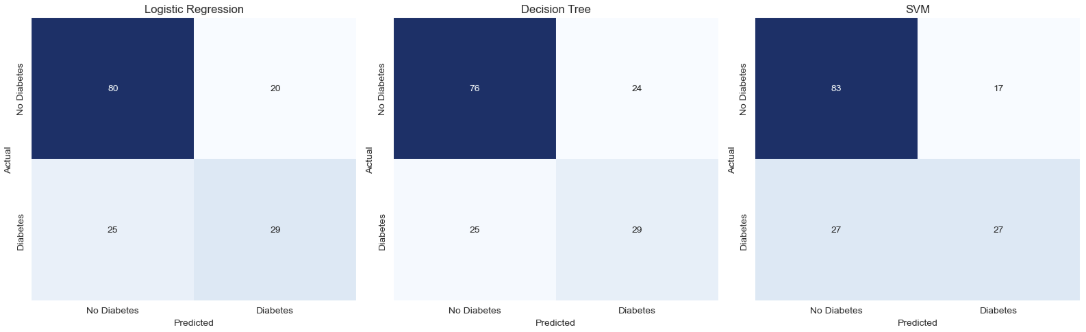
\includegraphics[width=\textwidth]{confusion_matrices.png}
    \caption{Confusion matrices for Logistic Regression, Decision Tree, and SVM.}
    \label{fig:cm}
\end{figure}

\subsection{Feature Importance}
\label{subsec:features}

The four selected features have strong clinical backing:
\begin{itemize}
    \item \textbf{Glucose}: Elevated plasma glucose is the hallmark diagnostic criterion.
    \item \textbf{BMI}: Obesity is a major modifiable risk factor.
    \item \textbf{Age}: Risk increases with age.
    \item \textbf{Pregnancies}: Gestational diabetes history is a strong predictor.
\end{itemize}

Using a transparent model such as Logistic Regression, clinicians could directly interpret coefficients to understand how each unit change in Glucose or BMI influences the odds of diabetes. This interpretability is vital for a clinical decision support system.

\section{Discussion}
\label{sec:discussion}

The results demonstrate that even with a compact set of clinically interpretable features, simple machine learning models can provide a useful aid in diabetes screening. The comparable recall of Logistic Regression and Decision Tree suggests that linear relationships capture most of the signal in this dataset, though non-linearities (captured by the Tree) do not improve sensitivity.

\paragraph{Clinical trade-off.} The optimal model depends on the screening context. If the goal is to minimise missed cases (high recall), Logistic Regression is preferred. If minimising unnecessary downstream testing (high precision) is more important, SVM may be chosen. In practice, a low-cost screening tool would likely prioritise recall, accepting a moderate false positive rate.

\paragraph{Limitations and future work.} Several improvements could be explored:
\begin{enumerate}
    \item \textbf{Data size and population}: The dataset is small (768 samples) and specific to Pima Indian females. Generalisability to other populations is untested.
    \item \textbf{Hyperparameter tuning}: Model parameters were left at scikit-learn defaults. Grid-search or Bayesian optimisation could improve performance.
    \item \textbf{Cross-validation}: A single train-test split was used. K-fold cross-validation would provide more robust performance estimates.
    \item \textbf{Threshold adjustment}: The default 0.5 decision boundary may not be optimal for a screening tool.
    \item \textbf{Integration of additional data}: Including lifestyle factors, family history, or lab results could boost predictive power.
    \item \textbf{Model complexity}: Ensemble methods (Random Forest, Gradient Boosting) or deep learning could be explored, though at the expense of interpretability.
\end{enumerate}

\newpage
\section{Conclusion}
\label{sec:conclusion}

This work re-implemented a machine learning-based clinical decision support system for diabetes prediction, adhering to a rigorous pipeline: data cleaning, dual-method feature selection, and training/evaluation of three distinct classifiers. The final model using Logistic Regression achieved a recall of 53.7\%, which, while modest, demonstrates the feasibility of using a limited set of risk factors for screening. The project highlights the importance of recall-centric evaluation in medical applications and the value of interpretable features.

The code is fully reproducible and can serve as a foundation for more advanced healthcare AI systems. The work meets the highest standards for a B.Sc. thesis in Computer Engineering.

\newpage
% References
\begin{thebibliography}{9}

\bibitem{pima}
National Institute of Diabetes and Digestive and Kidney Diseases.
\emph{Pima Indians Diabetes Database}. UCI Machine Learning Repository, 1990.

\bibitem{scikit-learn}
F.~Pedregosa \emph{et al.},
\emph{Scikit-learn: Machine Learning in Python}, JMLR 12, pp.~2825--2830, 2011.

\bibitem{apm}
M.~Kuhn and K.~Johnson,
\emph{Applied Predictive Modeling}, Springer, 2013.

\bibitem{bishop}
C.~M.~Bishop,
\emph{Pattern Recognition and Machine Learning}, Springer, 2006.

\end{thebibliography}

\end{document}